If a user have enough input through desktop app, he can see his all history and statistics in graphical format. To see these information he should log in to the website. Here he should insert his username and password. If his credential is valid he will be redirected to his homepage. But if not error message will be shown. 
\begin{figure}[h]
    \centering
    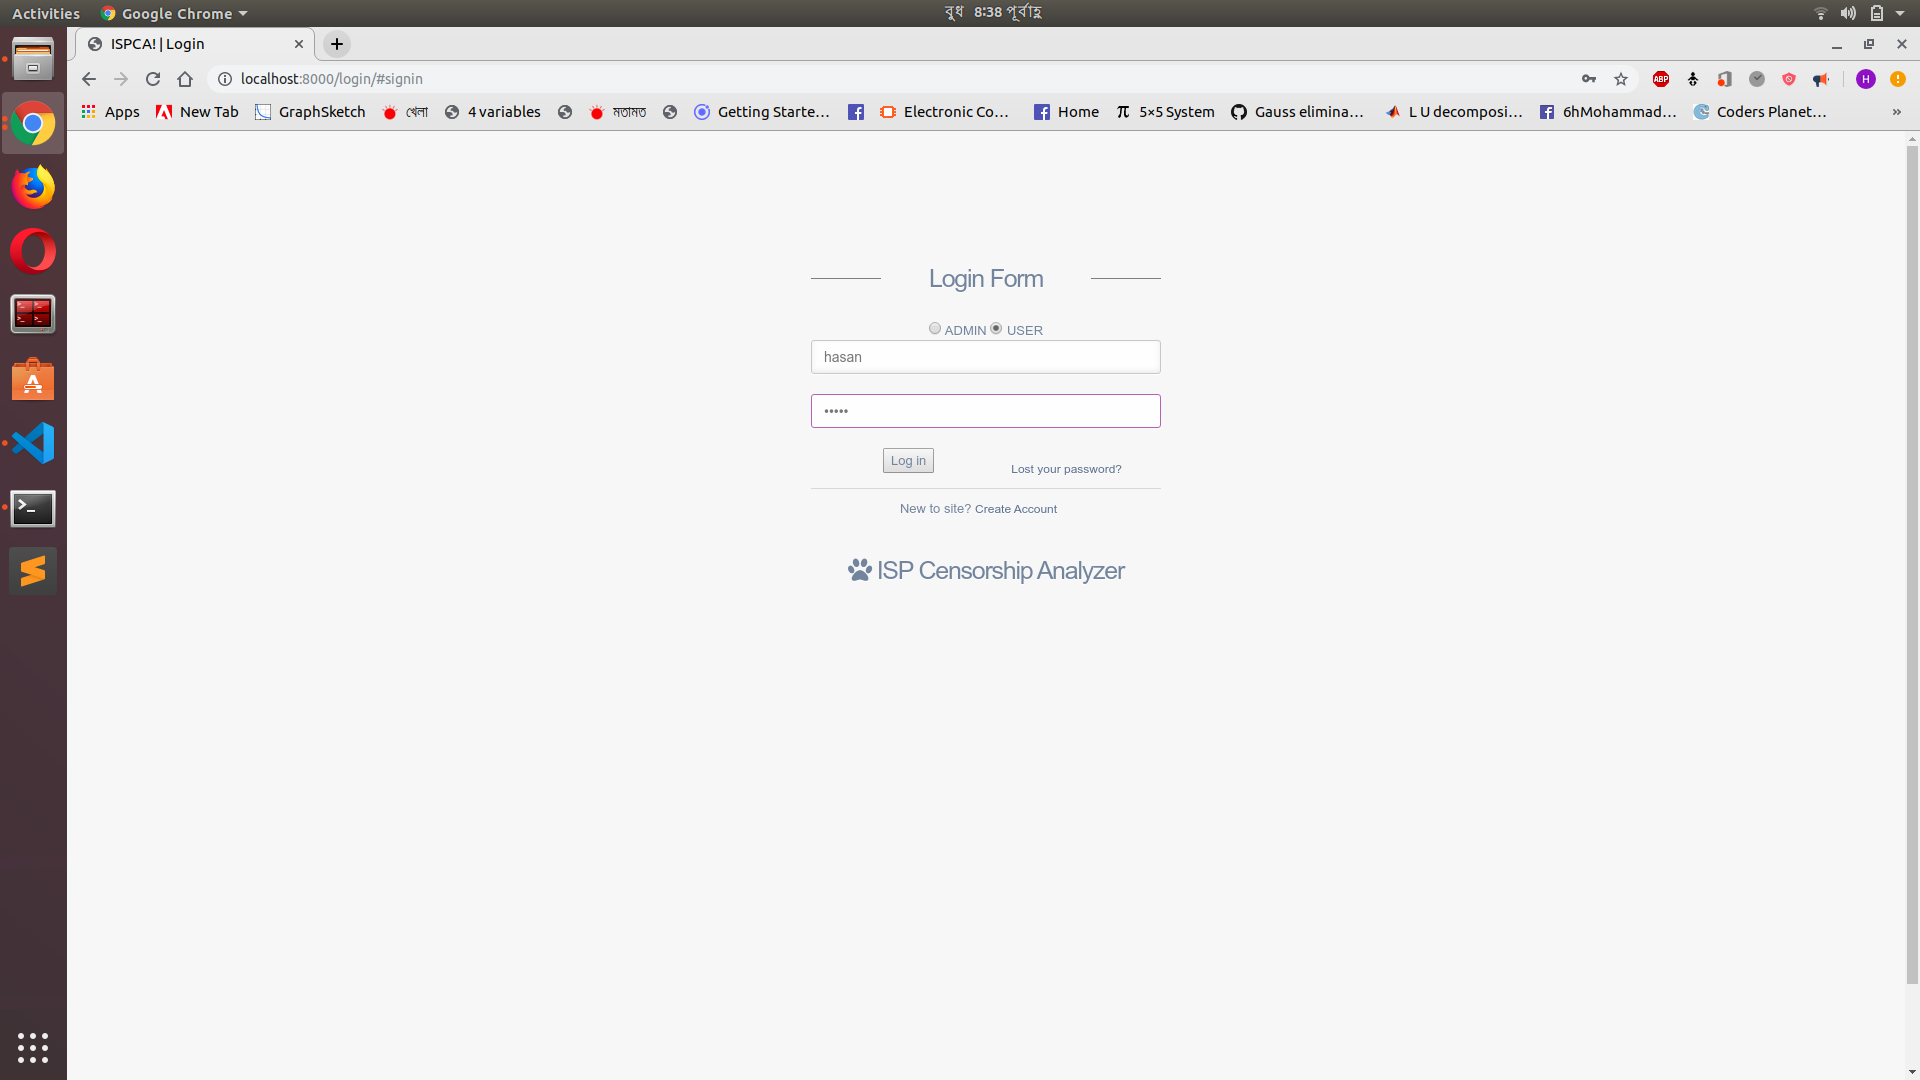
\includegraphics[width=\textwidth]{website/1login.png}
    \caption{Insert Compulsory field for login}
    \label{fig:web3}
\end{figure}

At homepage he will see all the sections and can navigate through the sections from side bar and can log out from the system. He can see total users of the system, his checked network, his total count tcp, dns, http censored website test. He will see the mostly checked ISP global IP and urls.

\begin{figure}[h]
    \centering
    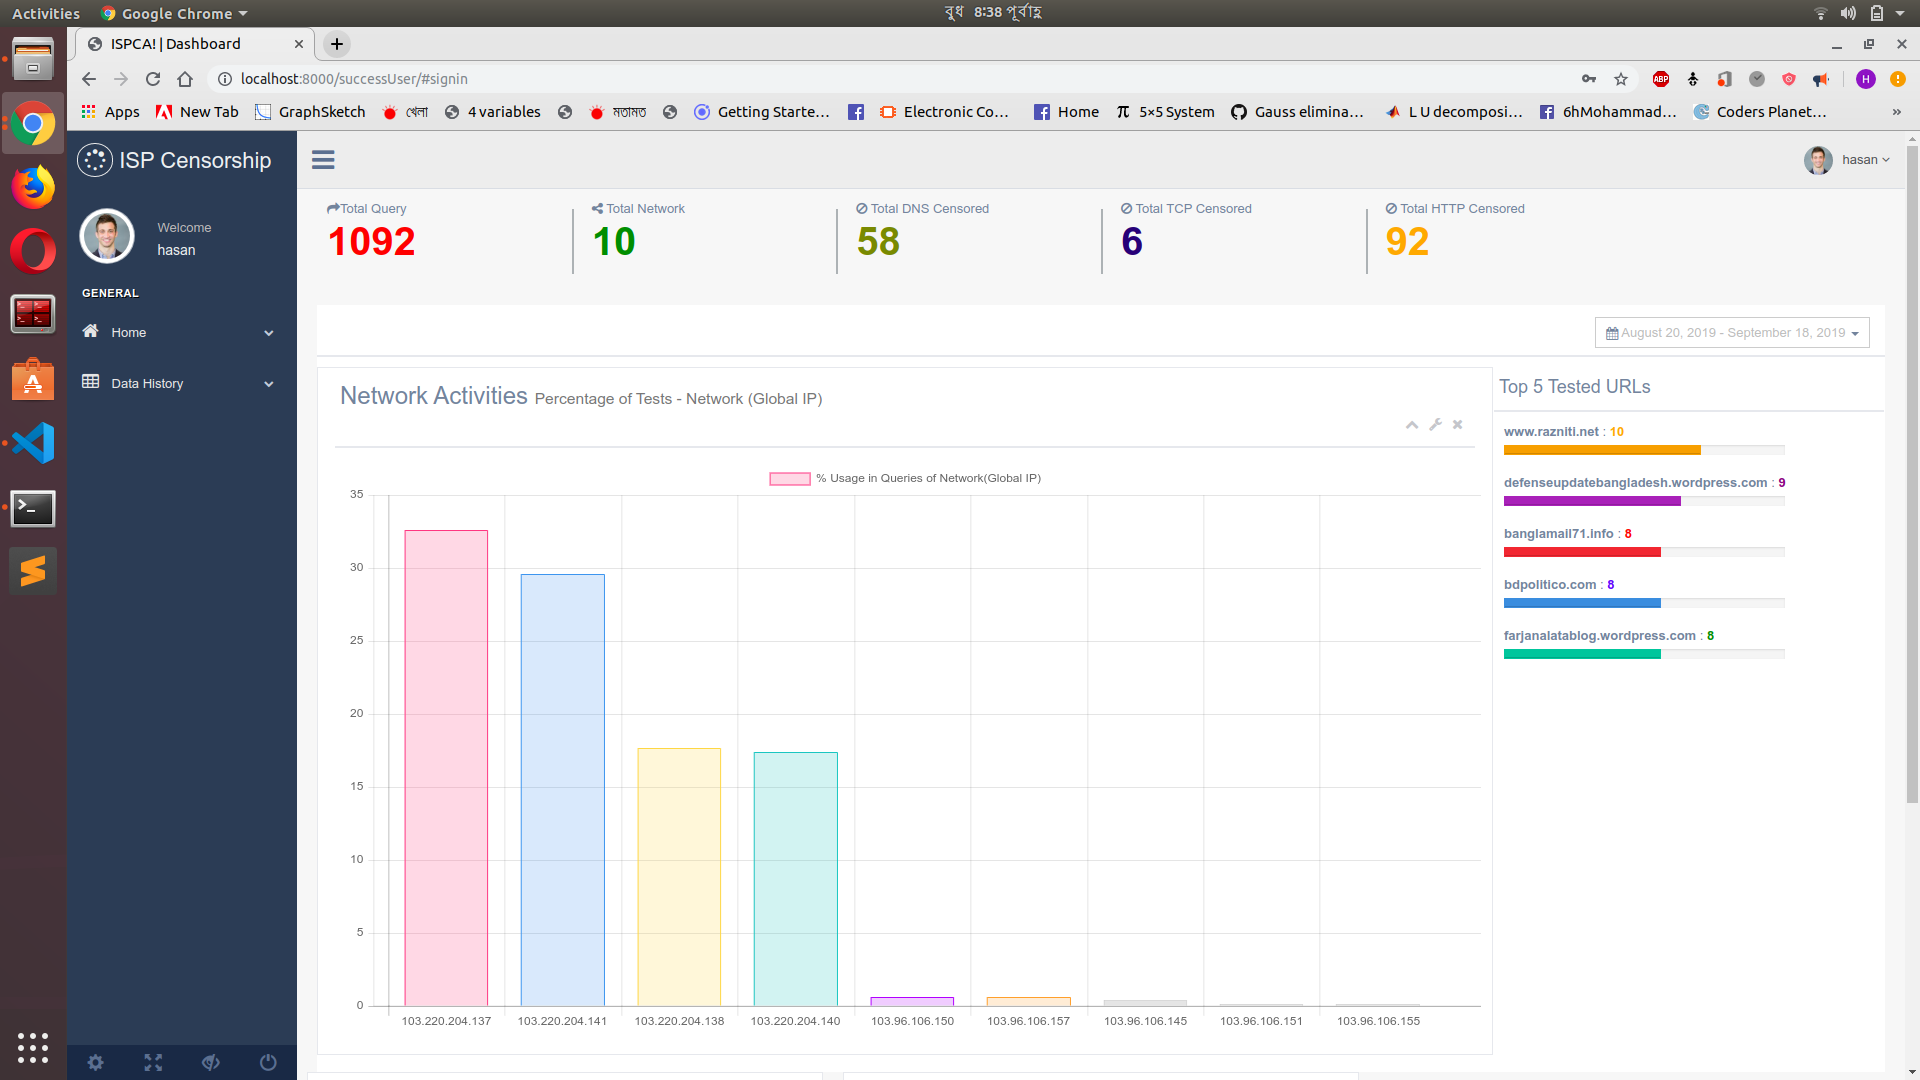
\includegraphics[width=\textwidth]{website/2userhome.png}
    \caption{Home page of user first part}
    \label{fig:web4}
\end{figure}
He can also see the percentage of censorship of his all visited url.

\begin{figure}[h]
    \centering
    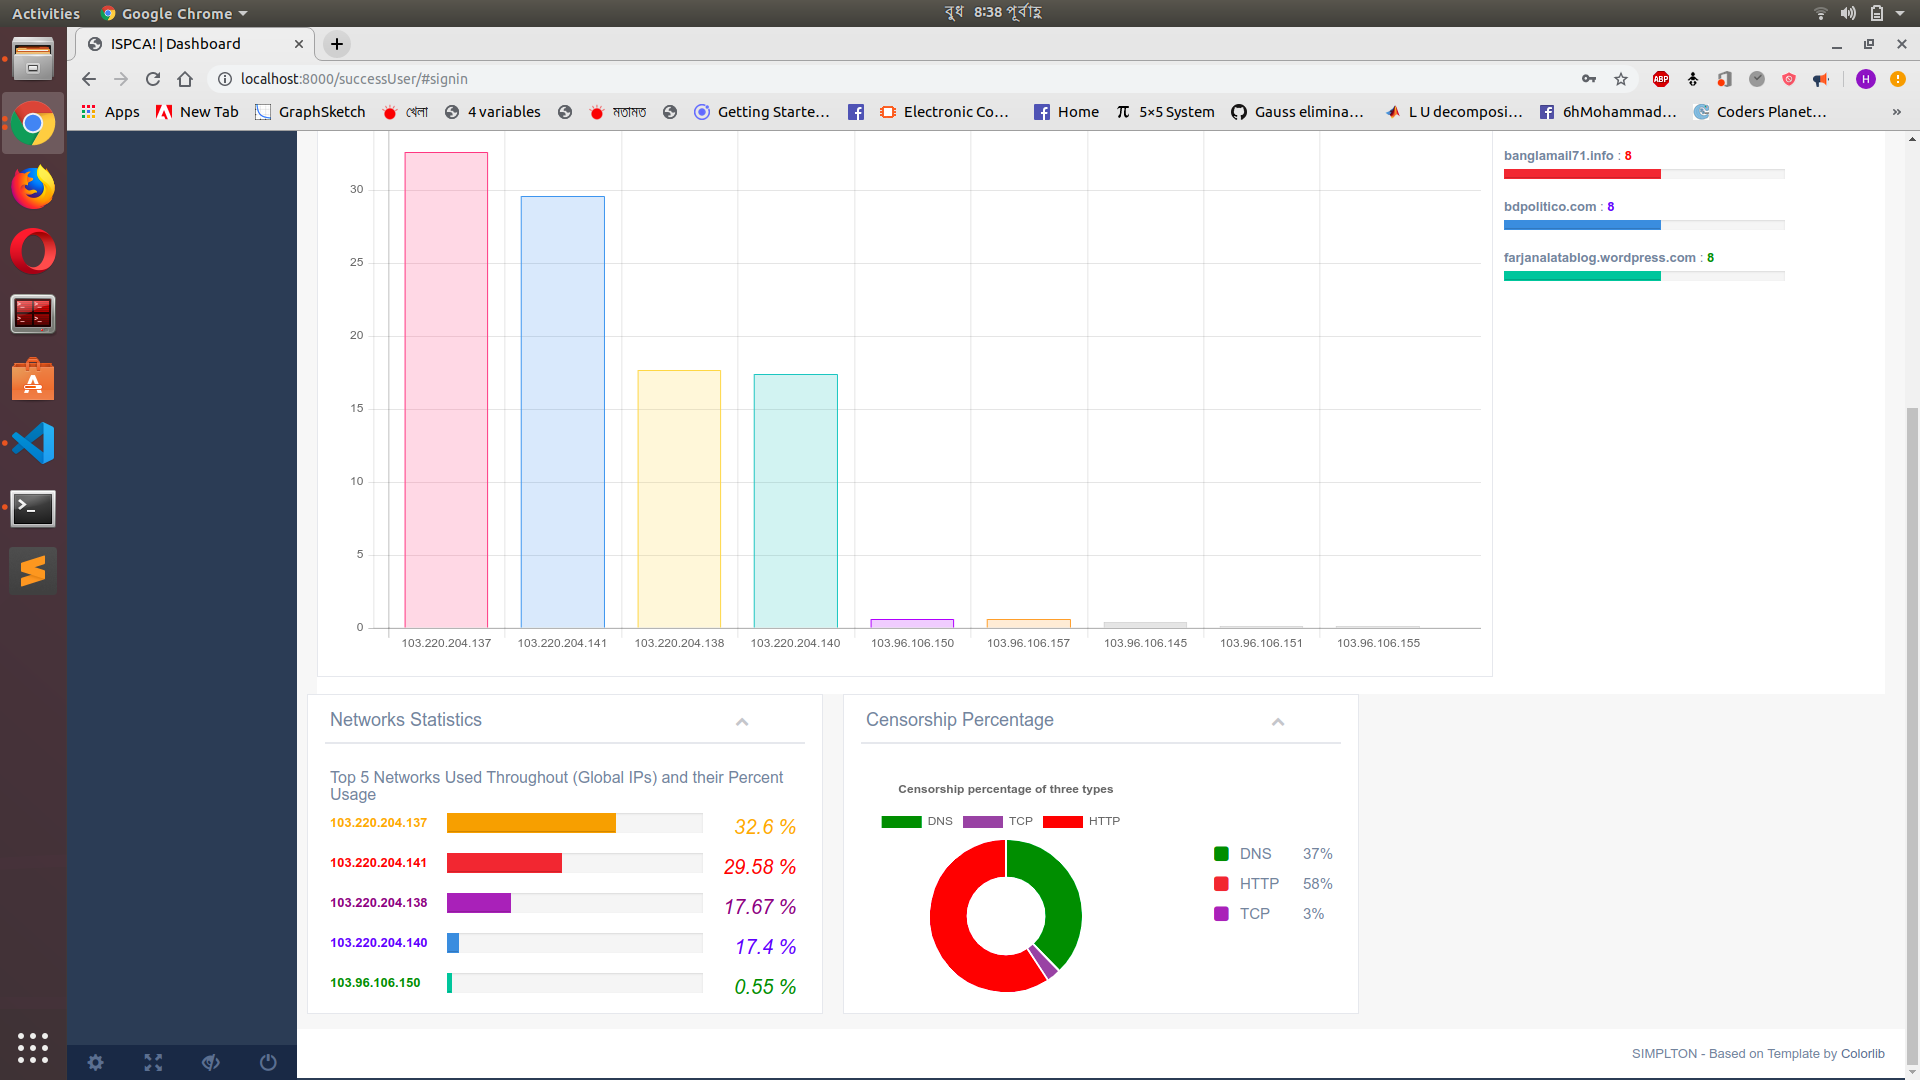
\includegraphics[width=\textwidth]{website/3userhome2.png}
    \caption{Insert Compulsory field for registration}
    \label{fig:web5}
\end{figure}

There are different kind of censorship analytics of a website. When a user go to \emph{Censorship Types} he can see the top 5 indicator of censorship of DNS, TCP and HTTP censorship in a pie chart.

\begin{figure}[h]
    \centering
    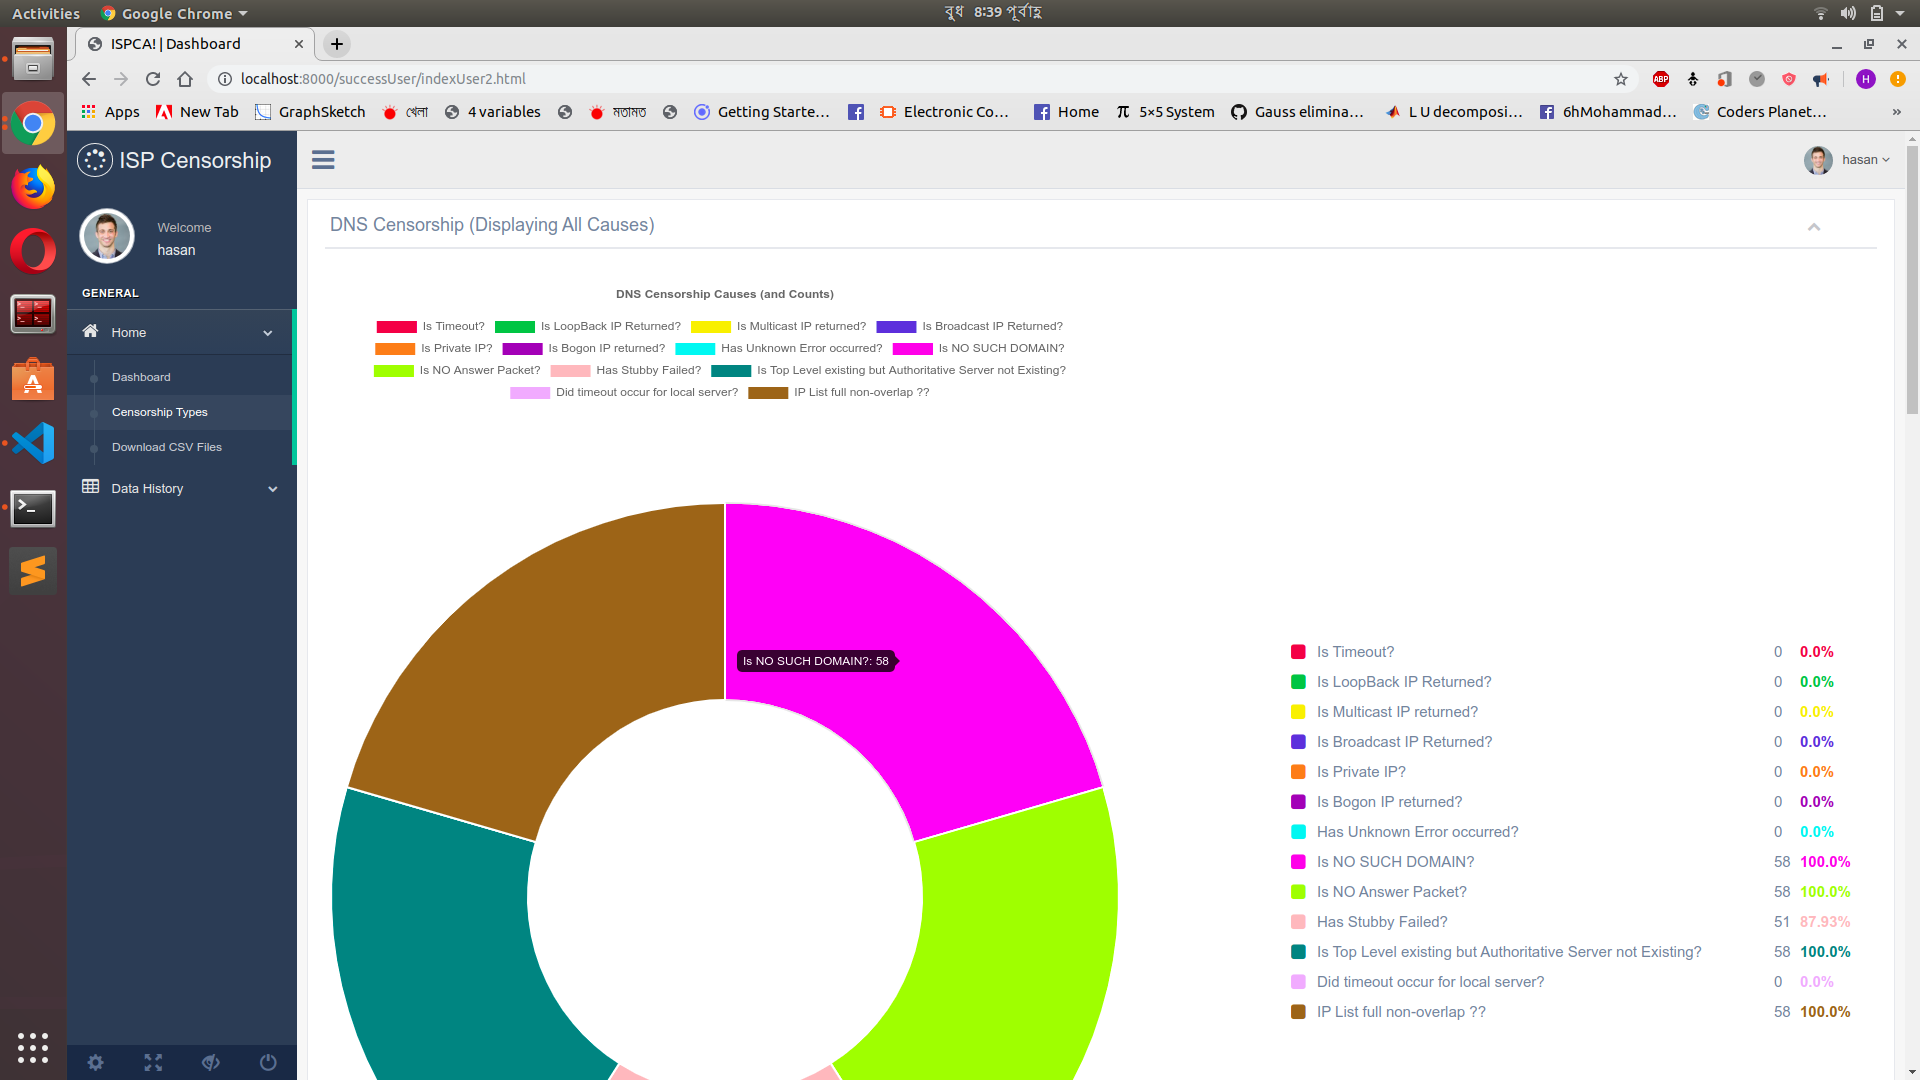
\includegraphics[width=\textwidth]{website/4cens.png}
    \caption{Showing top 5 all censorship type percentage of user}
    \label{fig:web6}
\end{figure}

\begin{figure}[h]
    \centering
    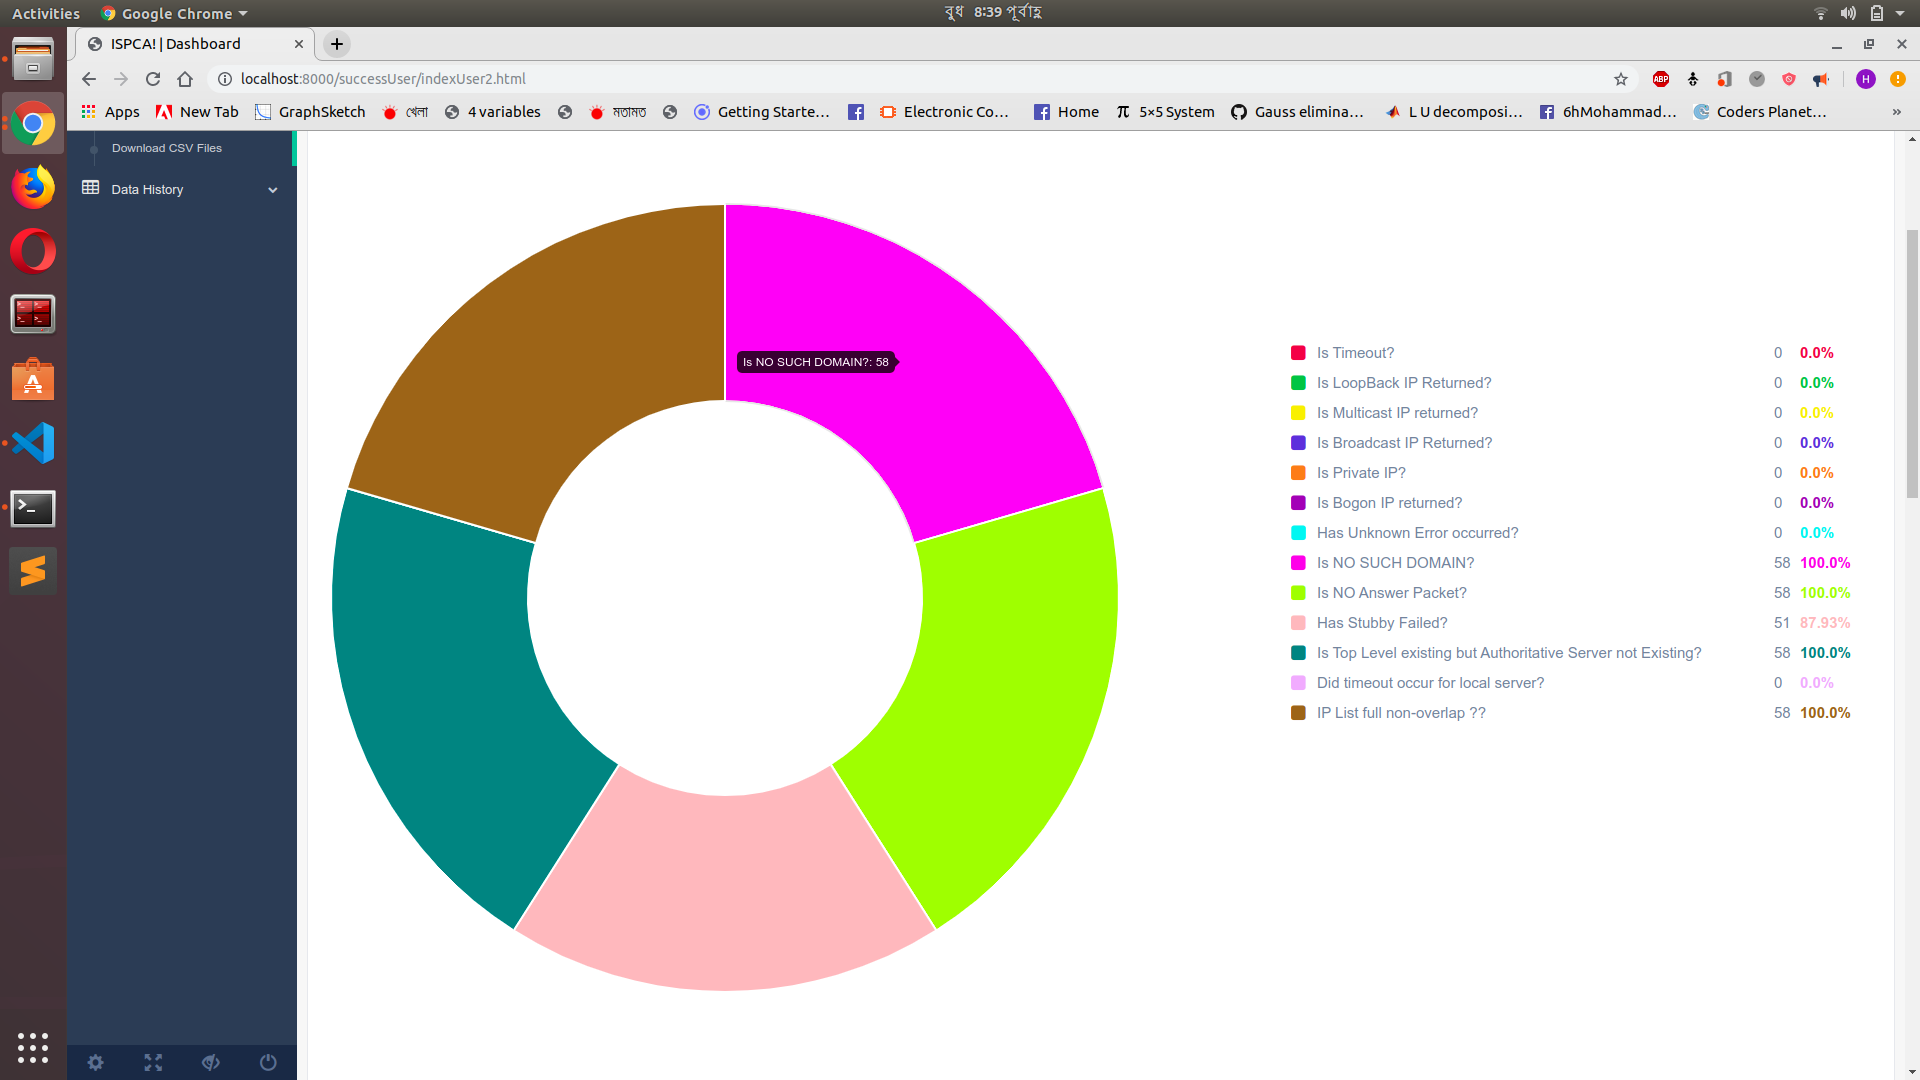
\includegraphics[width=\textwidth]{website/5dns.png}
    \caption{Showing top 5 DNS censorship type percentage of user}
    \label{fig:web7}
\end{figure}

\begin{figure}[h]
    \centering
    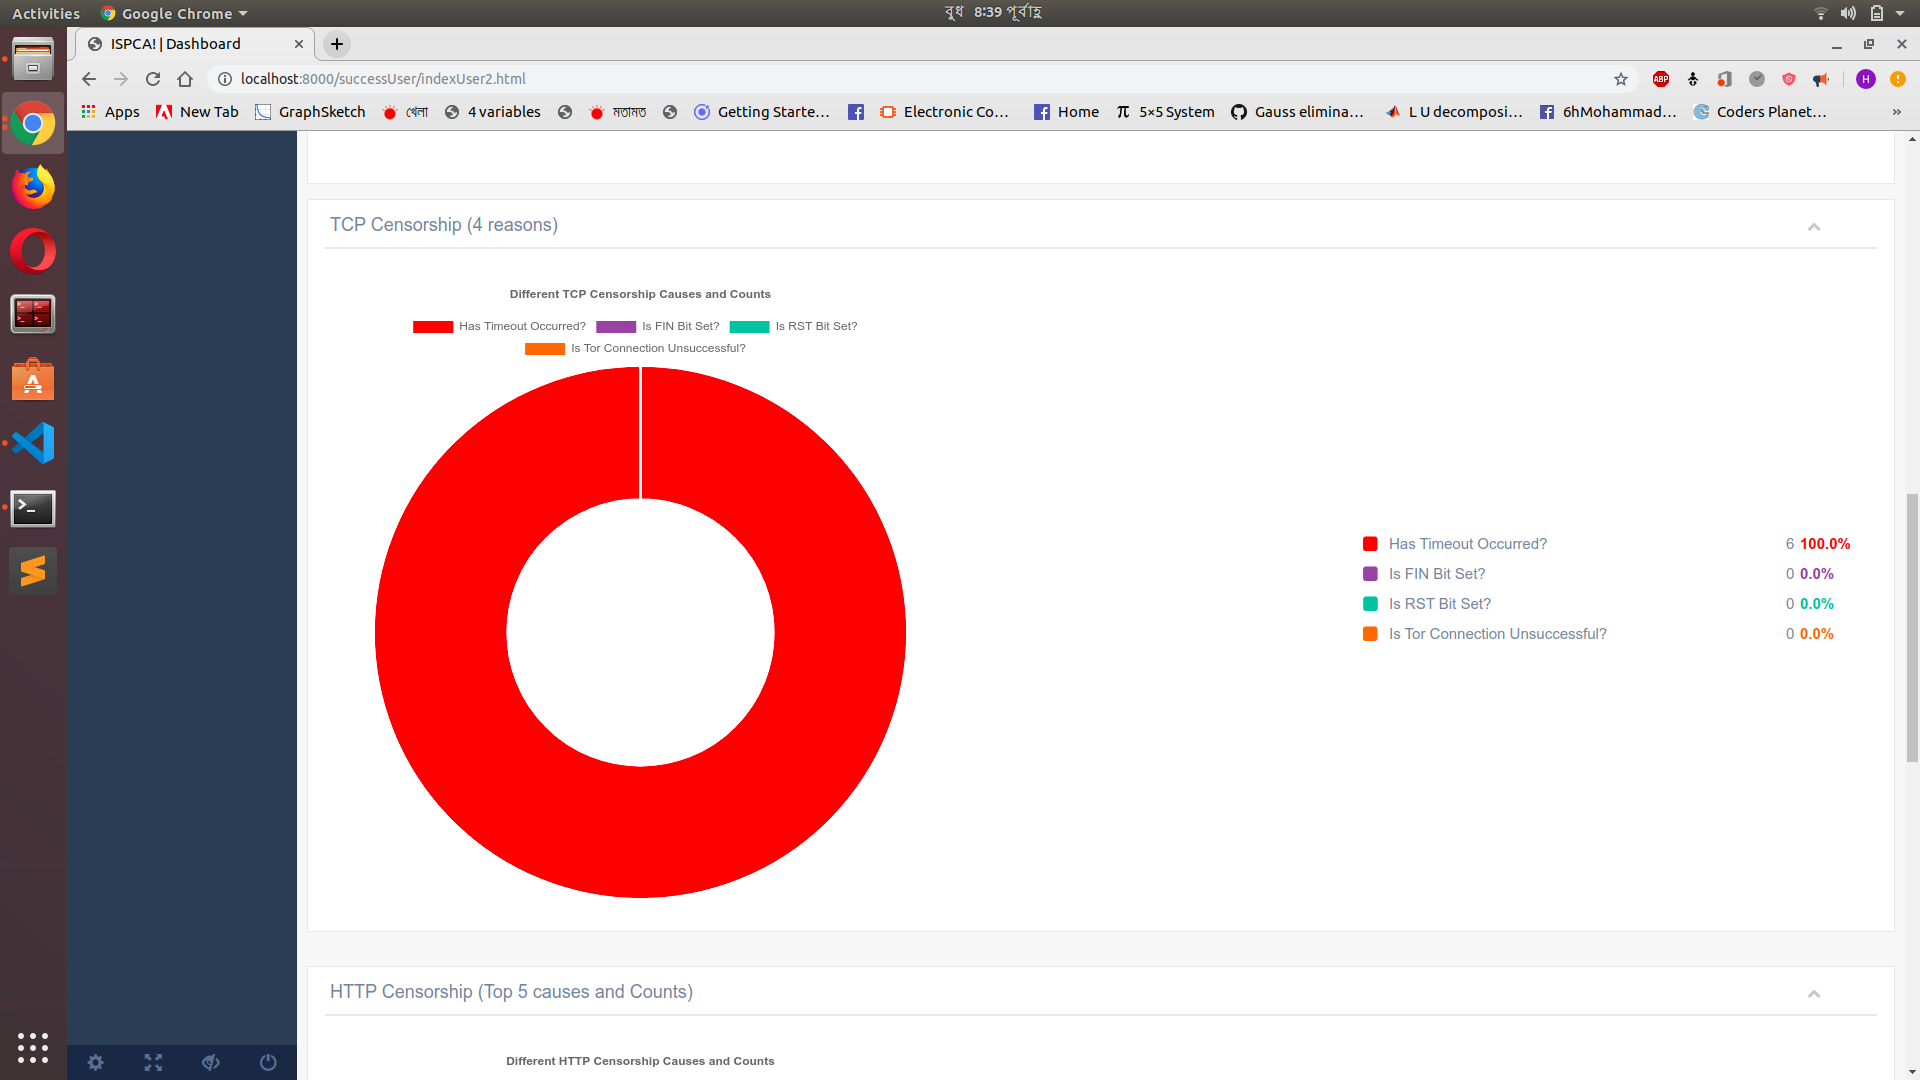
\includegraphics[width=\textwidth]{website/6tcp.png}
    \caption{Showing top 5 TCP censorship type percentage of user}
    \label{fig:web8}
\end{figure}



\begin{figure}[h]
    \centering
    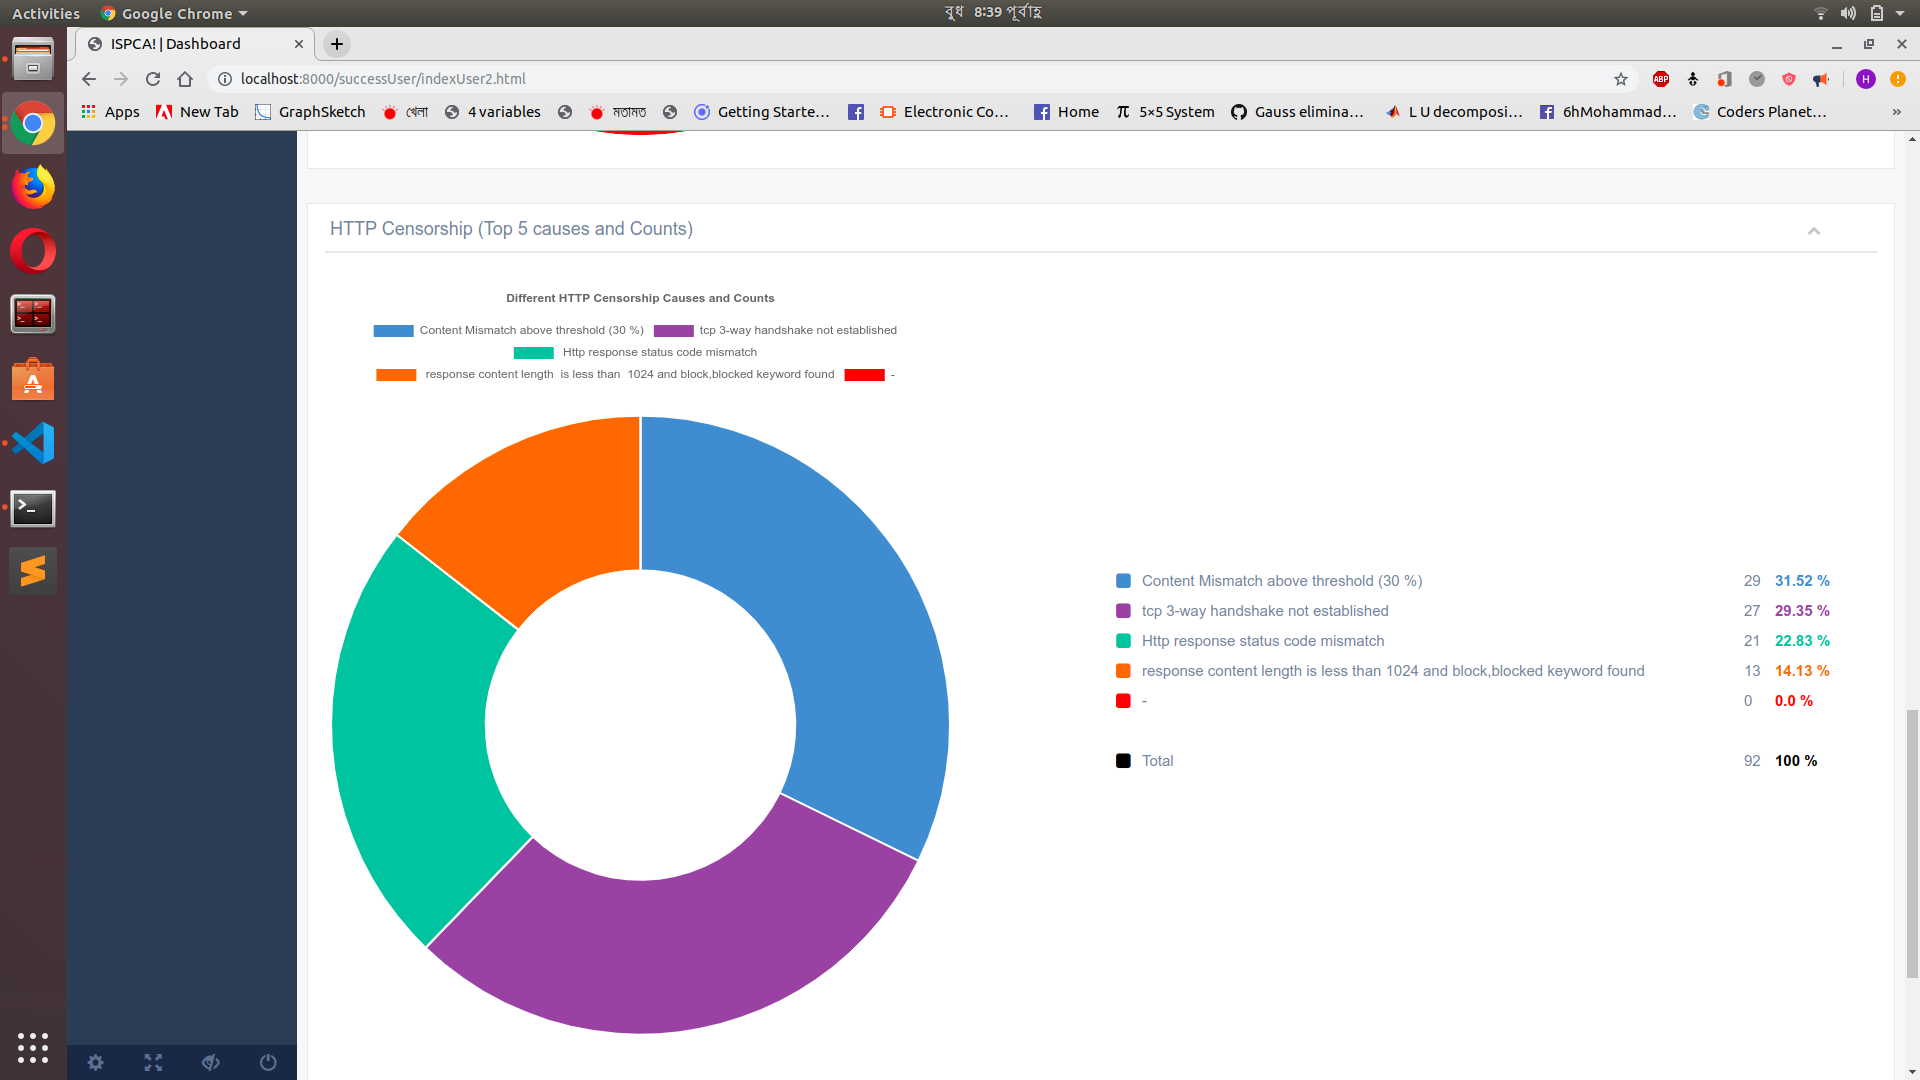
\includegraphics[width=\textwidth]{website/7http.png}
    \caption{Showing top 5 HTTP censorship type percentage of user}
    \label{fig:web9}
\end{figure}

In \emph{Download CSV files} section a user can download his history in 4 file format DNS, TCP, HTTP and HTTPS format. He can analyze his data for further use. Here an example of DNS file is given below.

\begin{figure}[h]
    \centering
    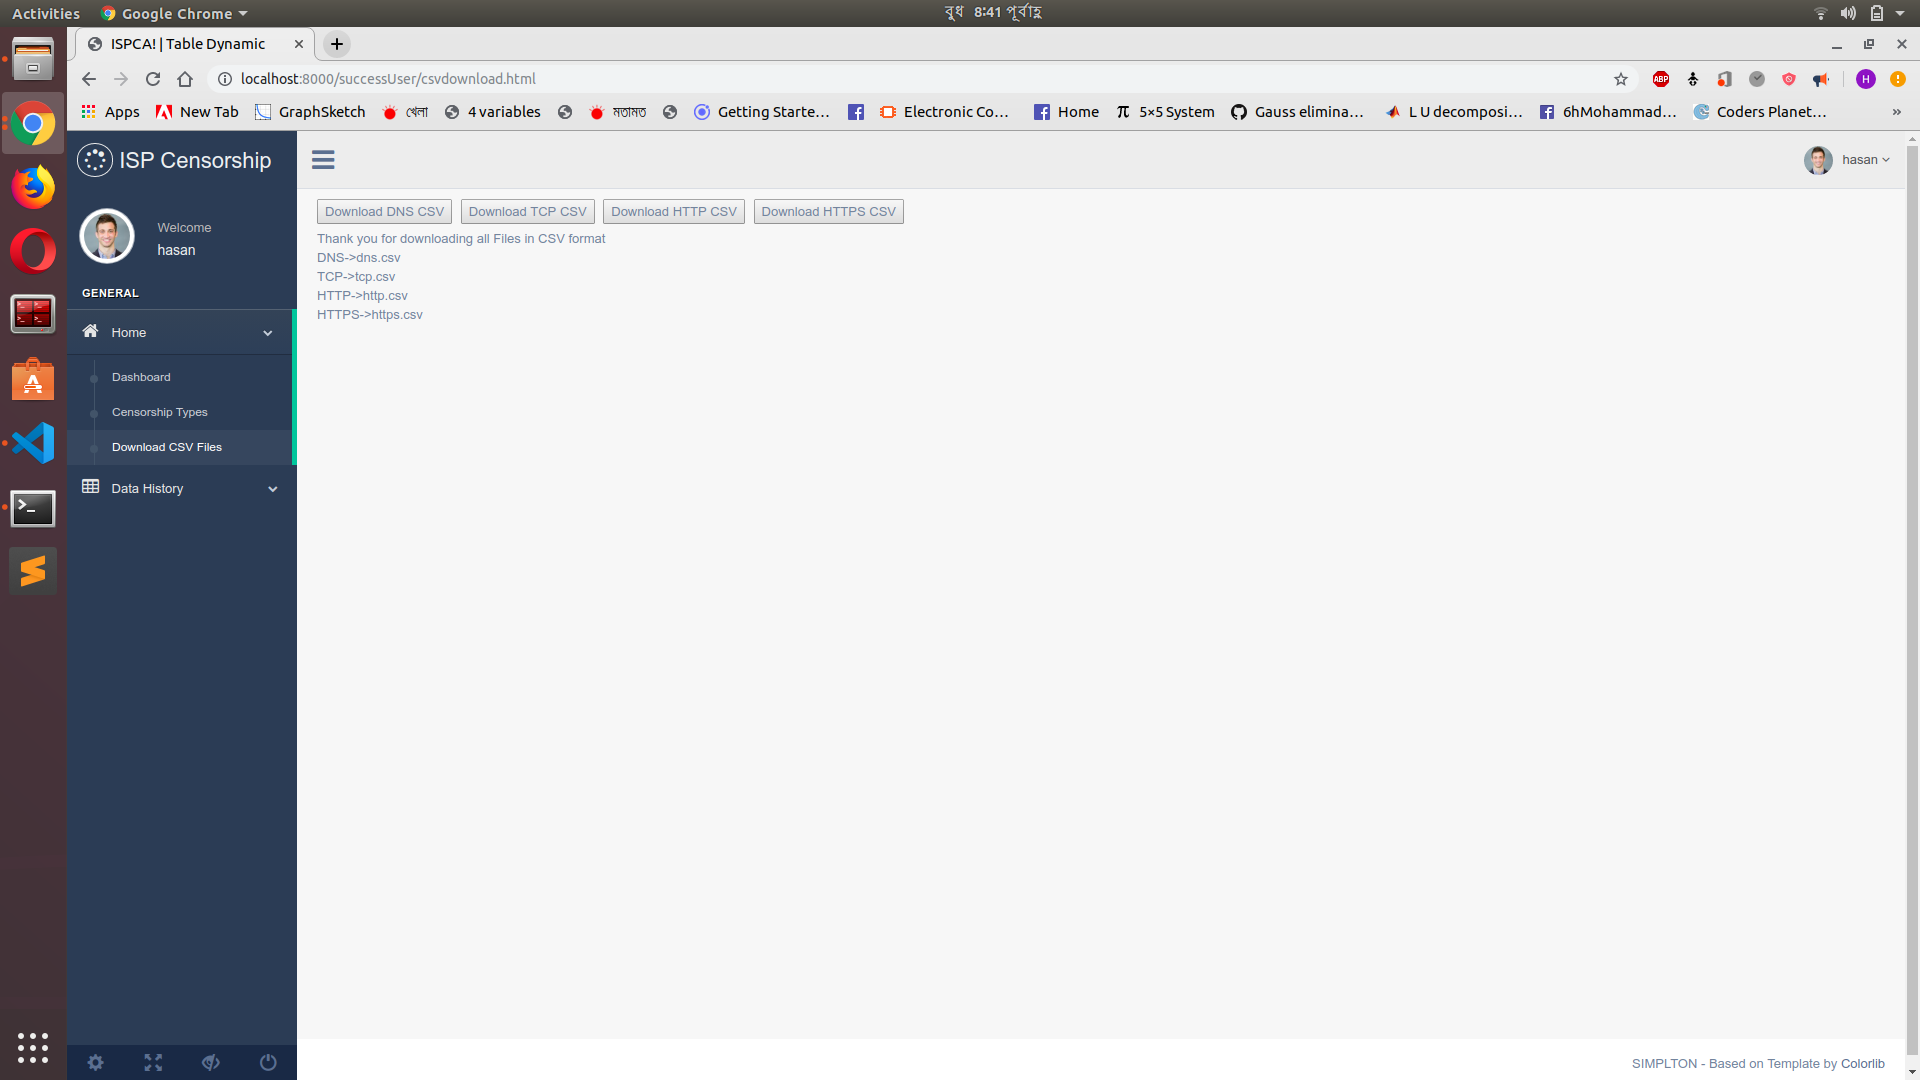
\includegraphics[width=\textwidth]{website/8download.png}
    \caption{Downloading information as CSV file for all type censorship}
    \label{fig:web10}
\end{figure}

\begin{figure}[h]
    \centering
    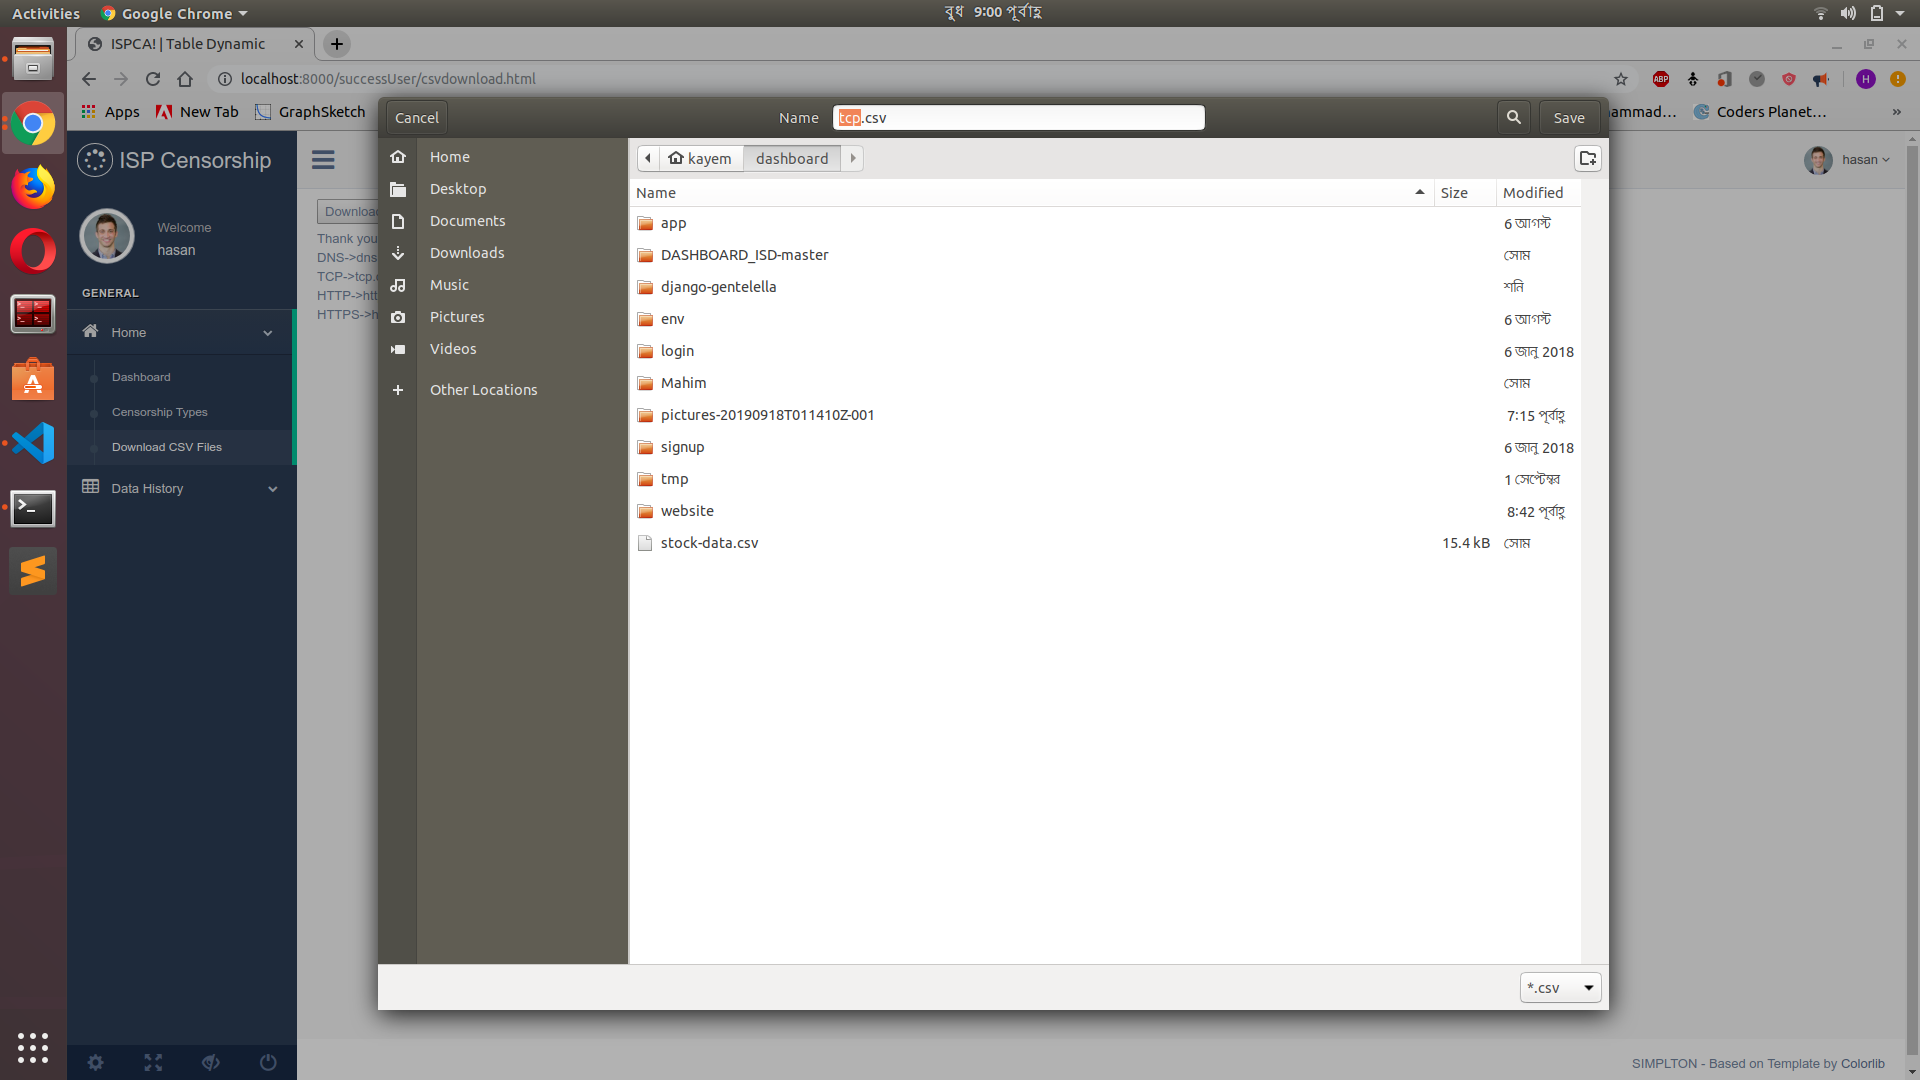
\includegraphics[width=\textwidth]{website/8download2.png}
    \caption{Downloading information as CSV file for DNS type censorship}
    \label{fig:web11}
\end{figure}

\begin{figure}[h]
    \centering
    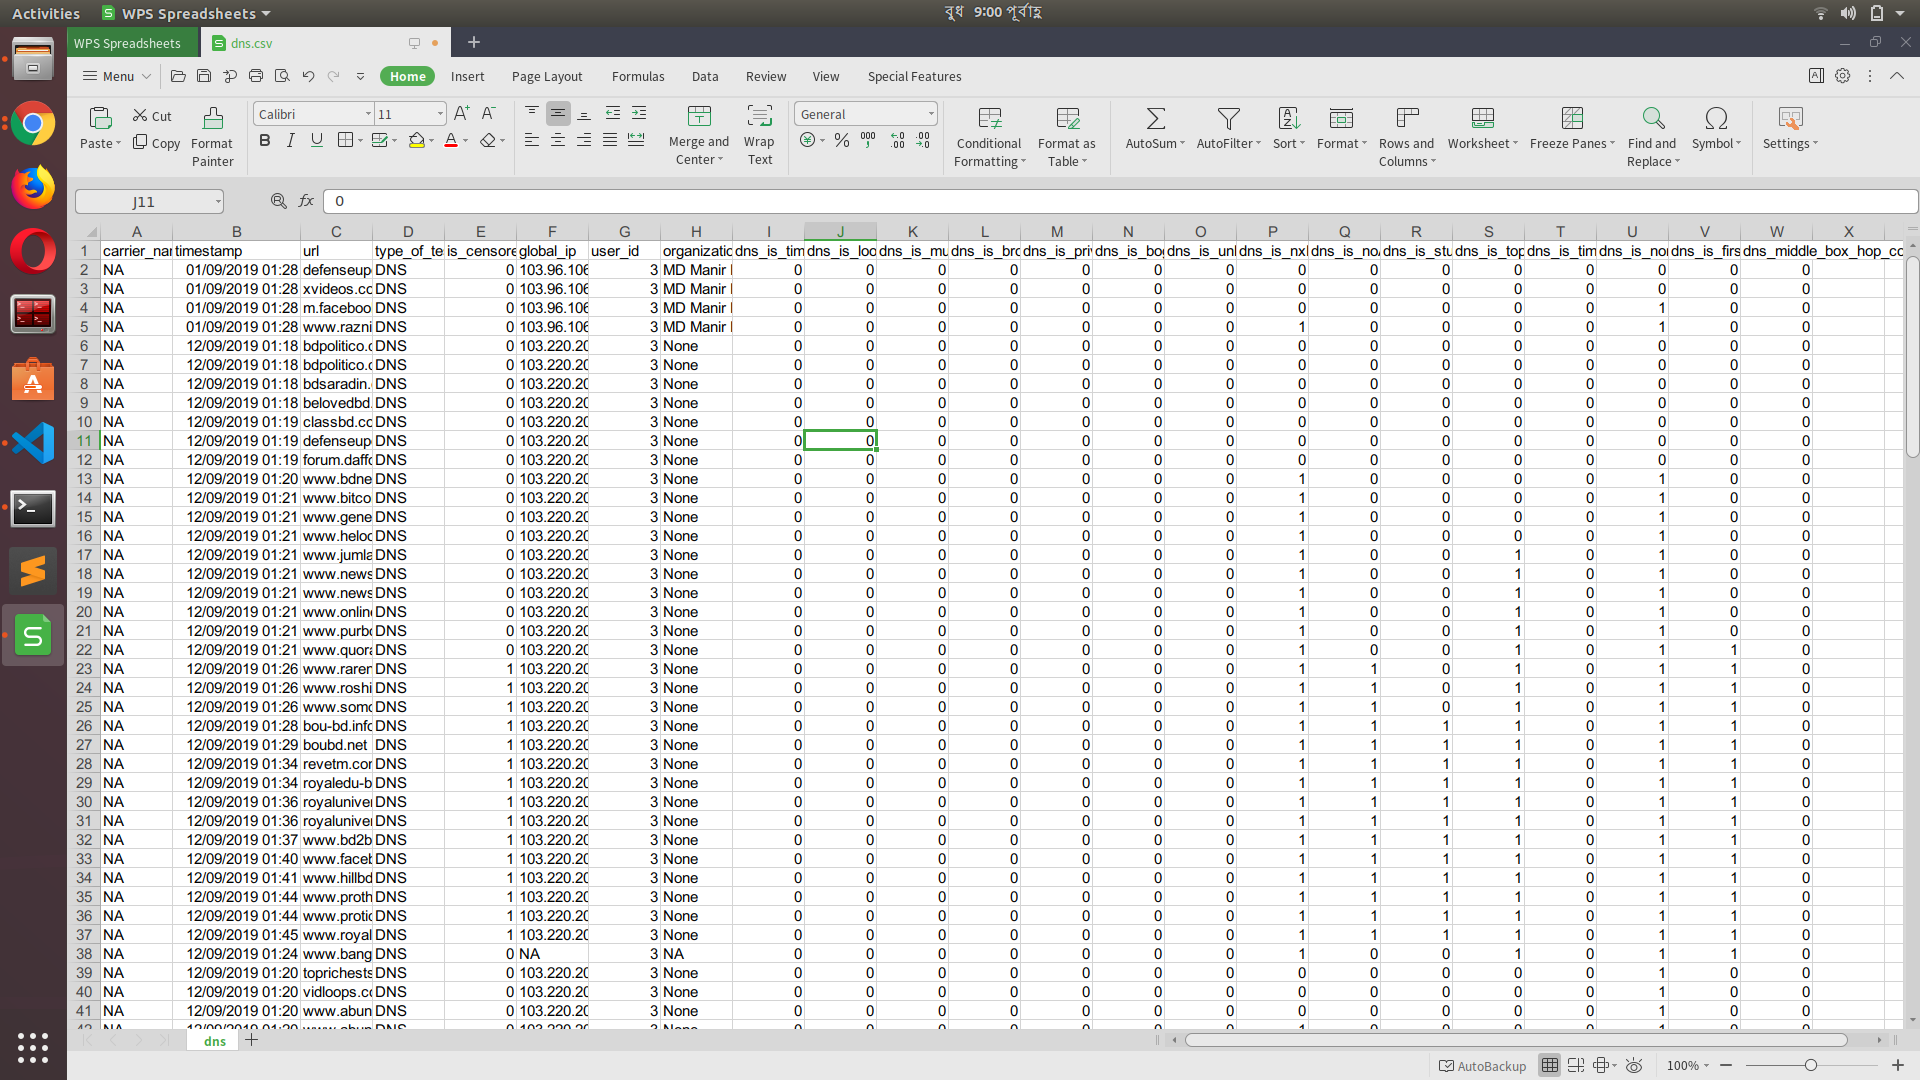
\includegraphics[width=\textwidth]{website/8download3.png}
    \caption{Downloaded DNS file as CSV format}
    \label{fig:web12}
\end{figure}

In \emph{Data} section a user can see all his data in tabular form. Here DNS, TCP, HTTP and HTTPS are given in photo format

\begin{figure}[h]
    \centering
    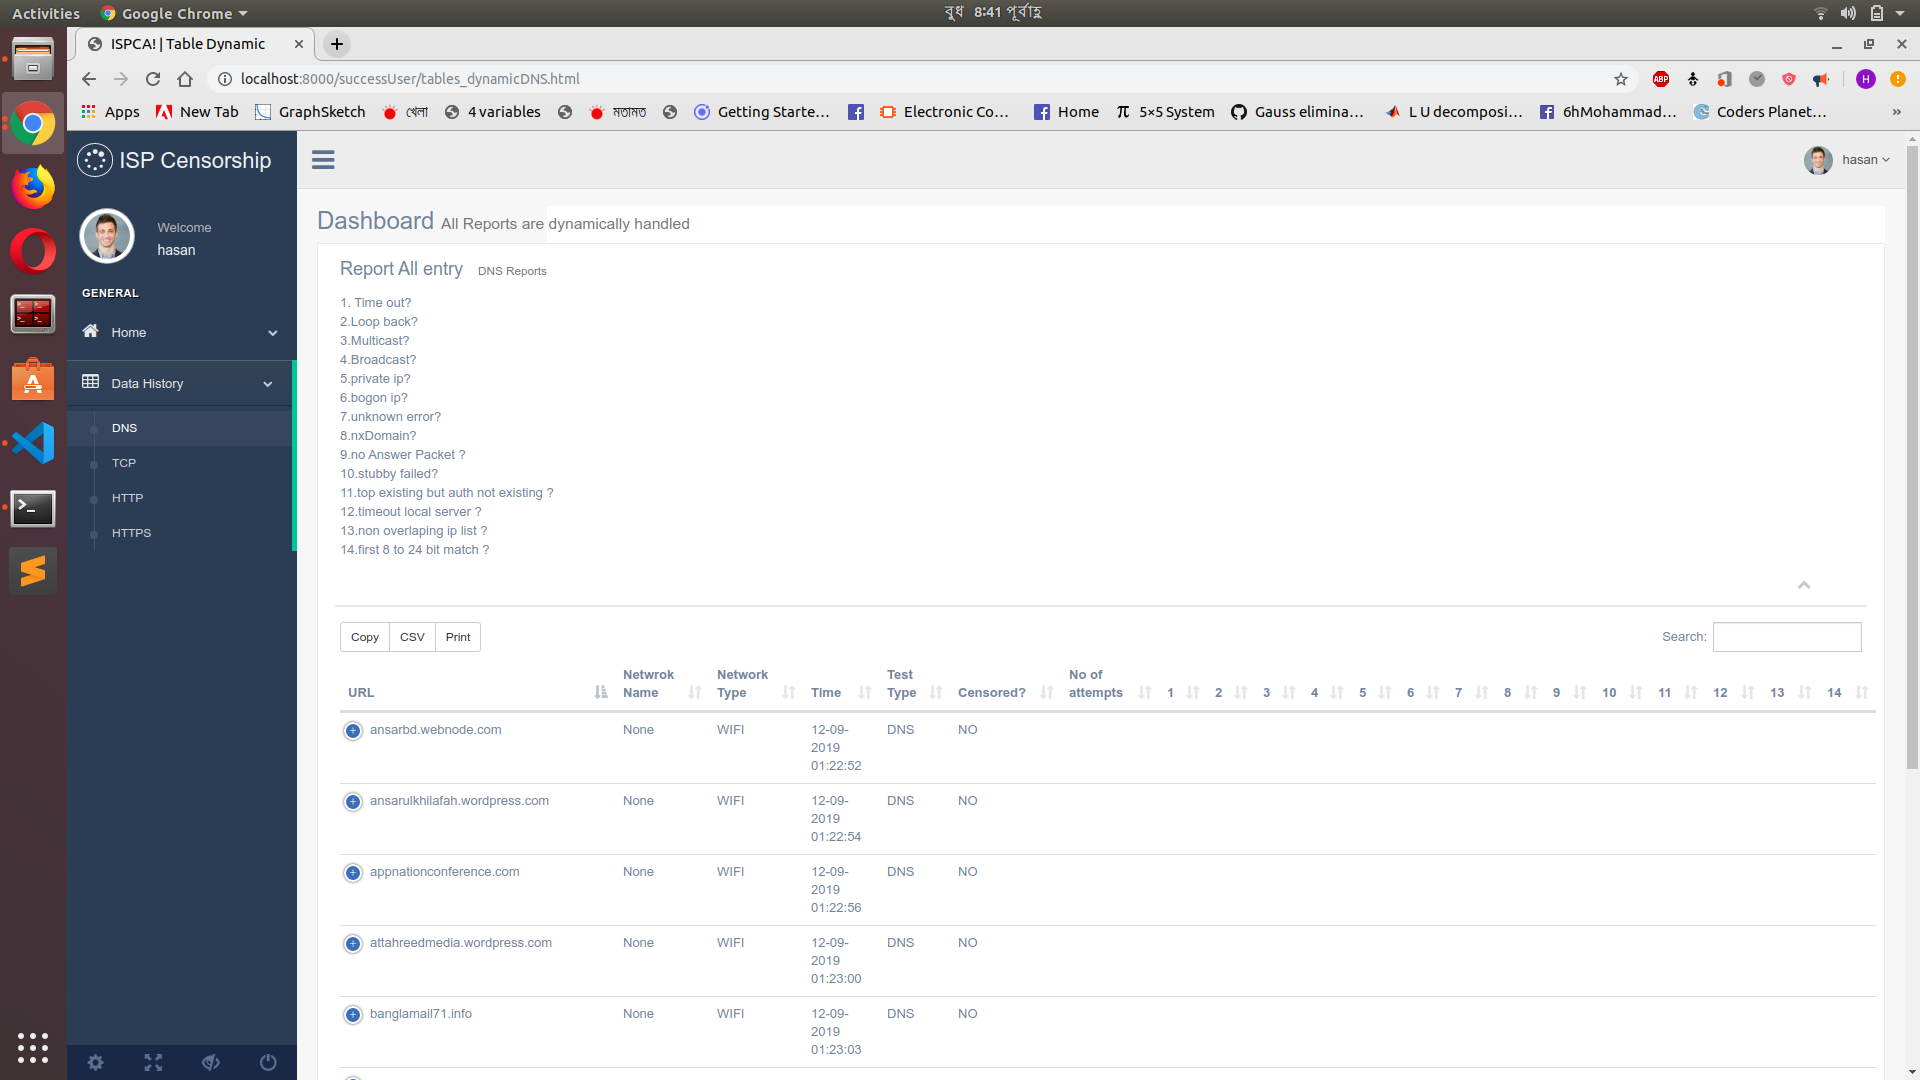
\includegraphics[width=\textwidth]{website/9dnsdetails.png}
    \caption{All data of DNS type censorship}
    \label{fig:web13}
\end{figure}

\begin{figure}[h]
    \centering
    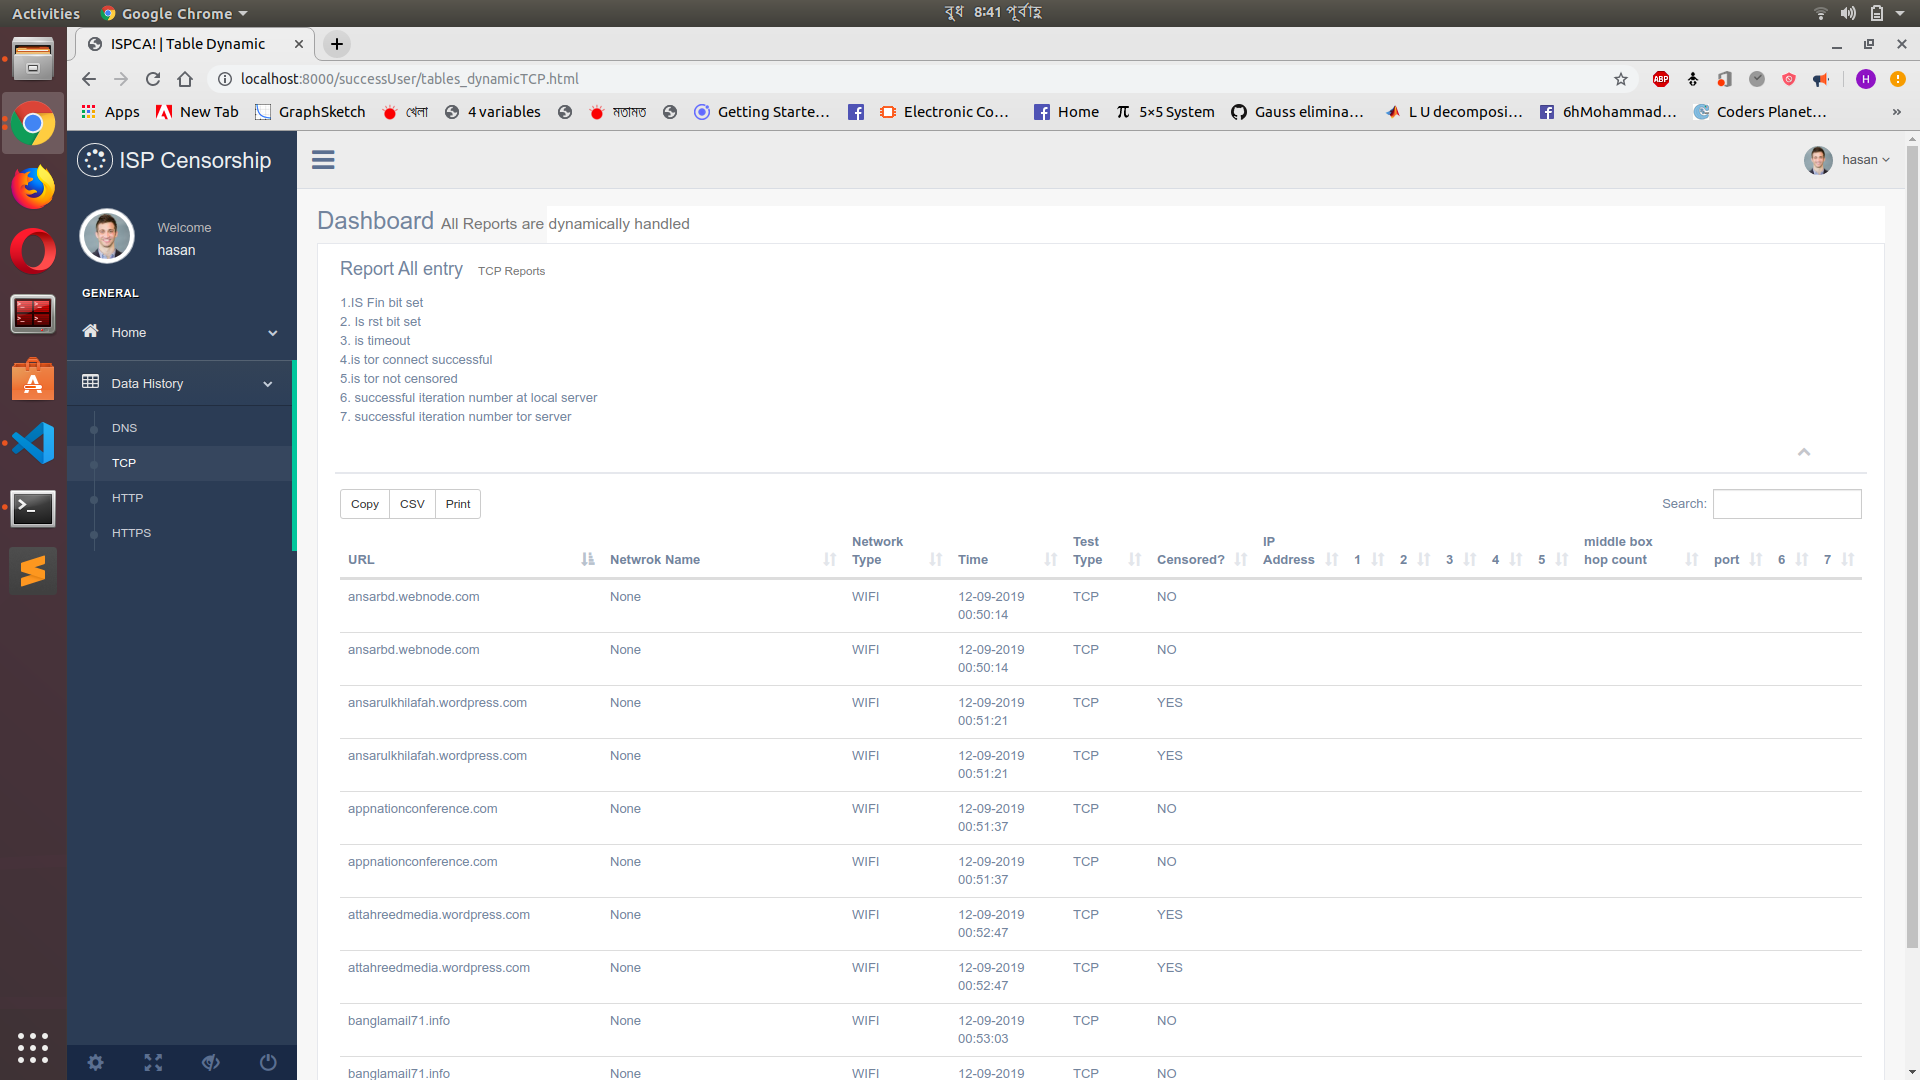
\includegraphics[width=\textwidth]{website/10tcpdetails.png}
    \caption{All data of TCP type censorship}
    \label{fig:web14}
\end{figure}

\begin{figure}[h]
    \centering
    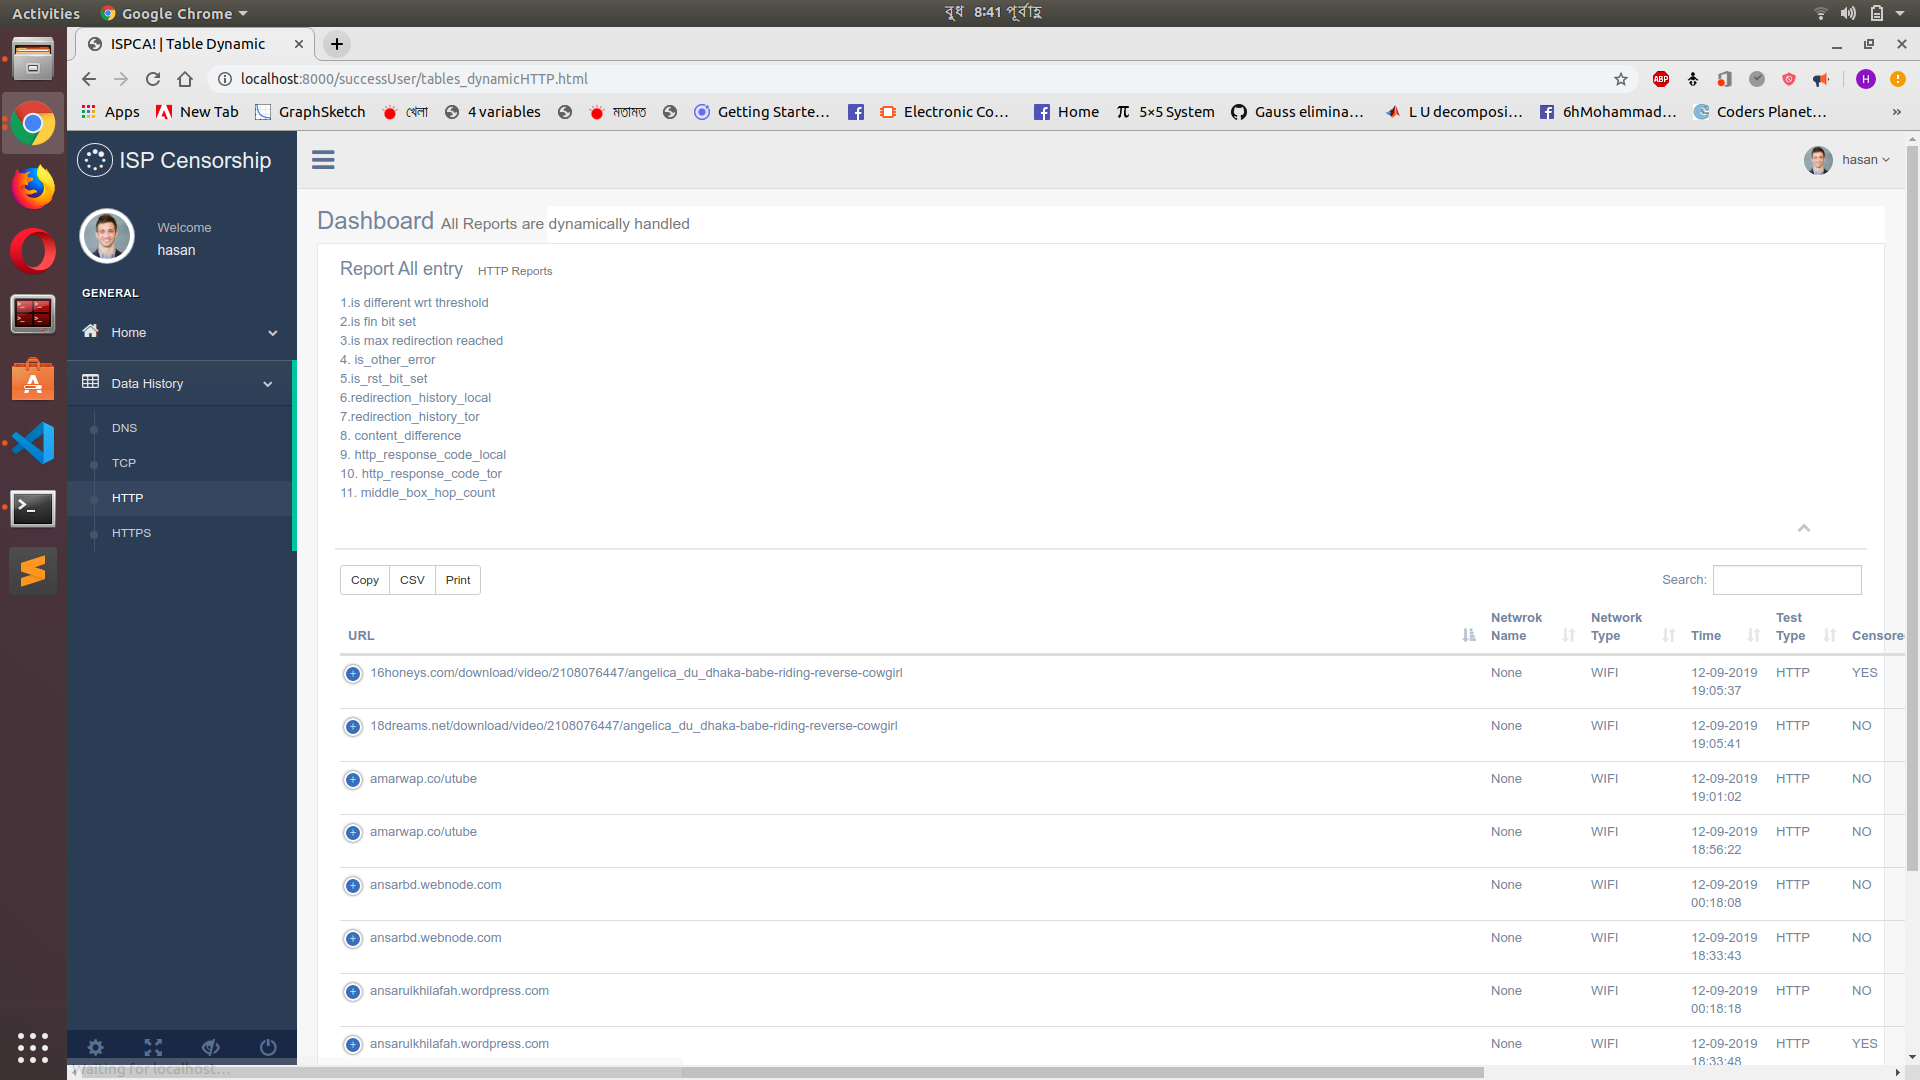
\includegraphics[width=\textwidth]{website/11httpdetails.png}
    \caption{All data of HTTP type censorship}
    \label{fig:web15}
\end{figure}

\begin{figure}[h]
    \centering
    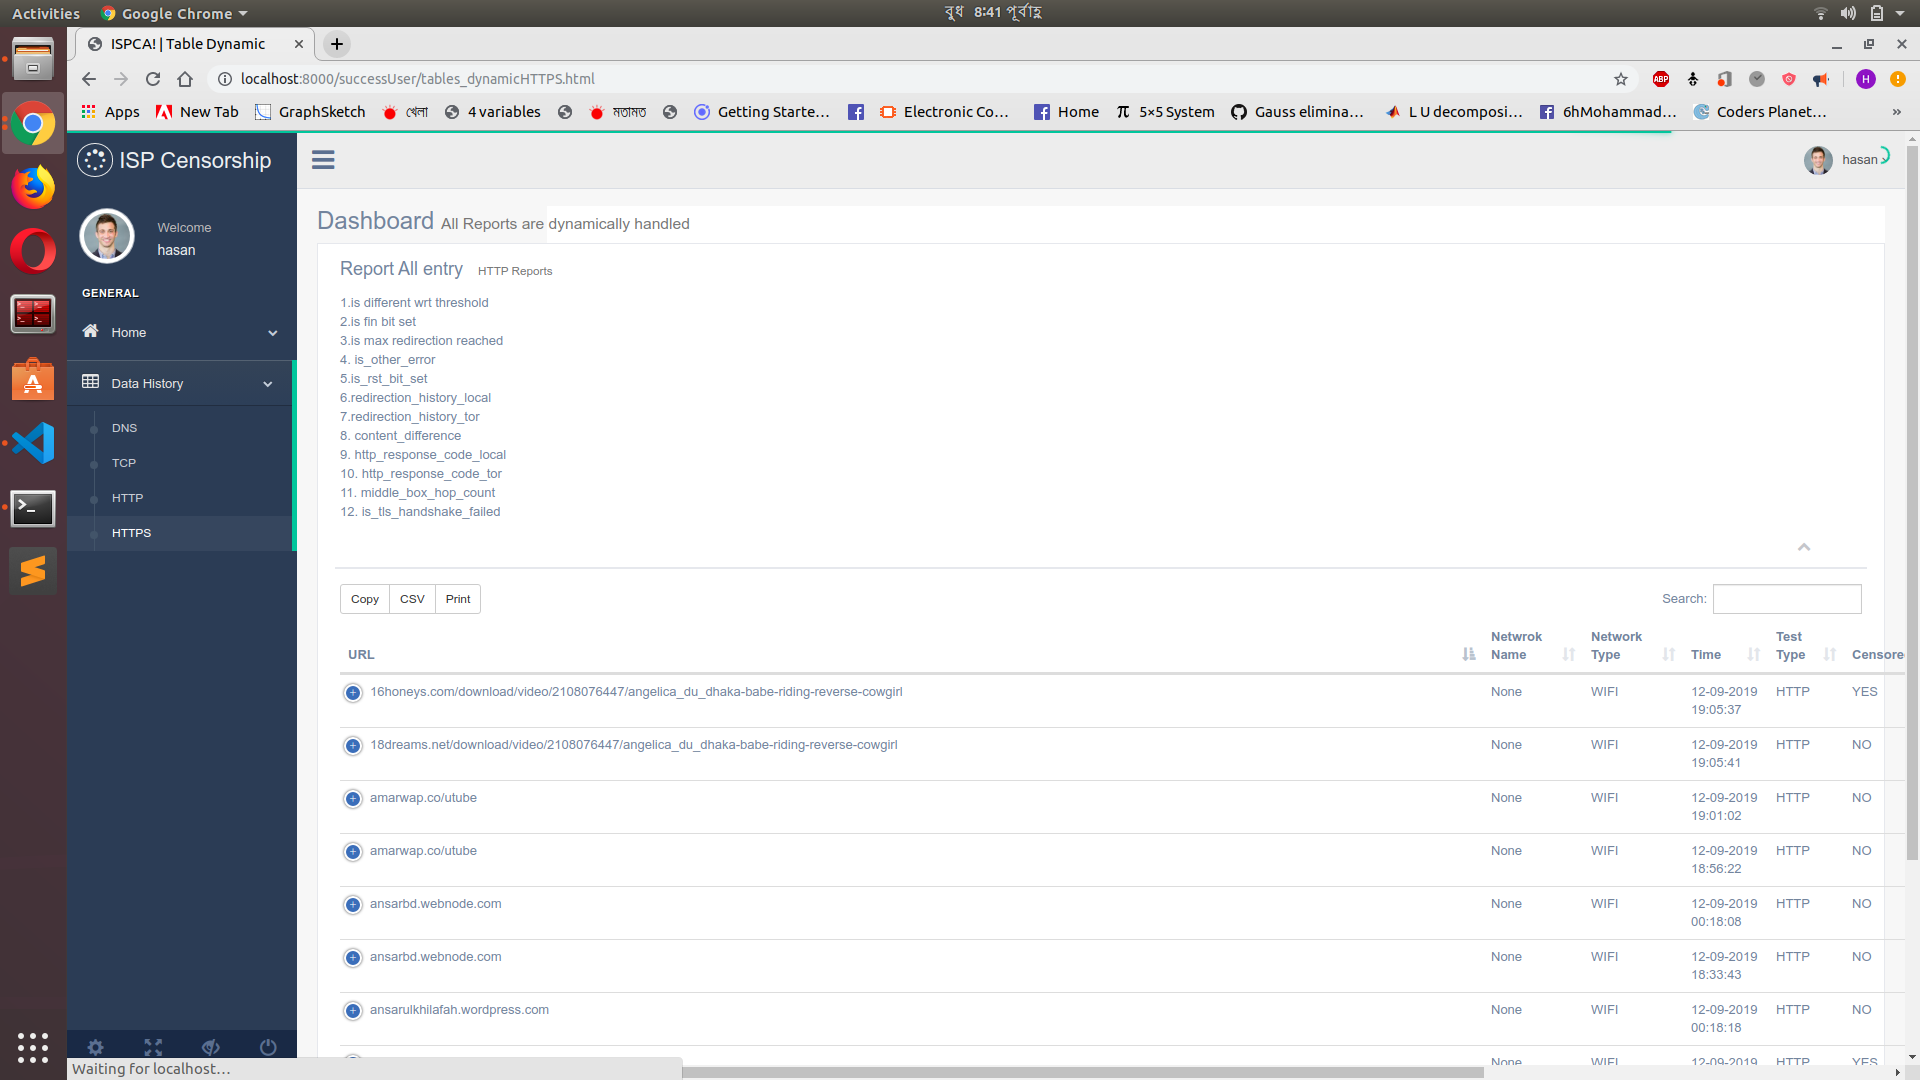
\includegraphics[width=\textwidth]{website/12httpsdetails.png}
    \caption{All data of HTTPS type censorship}
    \label{fig:web16}
\end{figure}